% !Mode:: "TeX:UTF-8"

\documentclass[12pt,oneside]{book}

\newlength{\textpt}
\setlength{\textpt}{12pt}
    
%========基本必备的宏包========%
\RequirePackage{calc,float,moresize}
%\RequirePackage[onehalfspacing]{setspace}
\linespread{1.5}
%1.3 onehalfspacing
%1.6 doublespacing

%===========加入目录 某章或某节=====%
\makeatletter

\newcommand{\addchtoc}[1]{
        \cleardoublepage
        \phantomsection
        \addcontentsline{toc}{chapter}{#1}}

\newcommand{\addsectoc}[1]{
        \phantomsection
        \addcontentsline{toc}{section}{#1}}

%===========全文基本格式==========%
\setlength{\parskip}{1.6ex plus 0.2ex minus 0.2ex}   %段落間距
\setlength{\parindent}{\textpt * \real{2}}
\RequirePackage{indentfirst} 

%=========页面设置=========%
\RequirePackage[a4paper, %a4paper size 297:210 mm
  bindingoffset=0mm,%裝訂線
  top=35mm,  %上邊距 包括頁眉
  bottom=30mm,%下邊距 包括頁腳
  inner=30mm,  %左邊距or inner
  outer=30mm,  %右邊距or  outer
  headheight=10mm,%頁眉
  headsep=15mm,%
  footskip=15mm,%
  marginparsep=0pt, %旁註與正文間距
  marginparwidth=0em,includemp=false% 旁註寬度計入width%旁註寬度
  ]{geometry}

%color
\RequirePackage[table,svgnames]{xcolor}

%================字體================%
%设置数学字体
\RequirePackage{amssymb,amsmath}
\RequirePackage{stmaryrd}
\everymath{\displaystyle}

\RequirePackage{fontspec}
%設置英文字體
\setmainfont[Mapping=tex-text]{DejaVu Serif}
\setsansfont[Mapping=tex-text]{DejaVu Sans}
\setmonofont[Mapping=tex-text]{DejaVu Sans Mono}


%中文環境
\RequirePackage[]{xeCJK}
\xeCJKsetup{PunctStyle=plain}
\setCJKmainfont[FallBack=DejaVu Serif, ItalicFont=KaiTi]{Source Han Serif CN}
\setCJKsansfont[FallBack=DejaVu Sans]{Source Han Sans CN}
\setCJKmonofont[FallBack=DejaVu Sans Mono]{KaiTi}


%%===============中文化=========%
\renewcommand\contentsname{目~录}
\renewcommand\listfigurename{插图目录}
\renewcommand\listtablename{表格目录}
\renewcommand\bibname{参~考~文~献}
\renewcommand\indexname{索~引}
\renewcommand\figurename{图}
\renewcommand\tablename{表}
\renewcommand\partname{部分}
\renewcommand\appendixname{附录}
\renewcommand{\today}{\number\year{}年\number\month{}月\number\day{}日}


%=======页眉页脚格式=========%
\RequirePackage{fancyhdr}   %頁眉頁腳
\RequirePackage{zhnumber}  %计数器中文化
\pagestyle{fancy}
\renewcommand{\sectionmark}[1]
{\markright{第\zhnumber{\arabic{section}}节~~#1}{}}

\fancypagestyle{plain}{%
    \fancyhf{}
    \renewcommand{\headrulewidth}{0pt}
    \renewcommand{\footrulewidth}{0pt}
    \fancyhf[HR]{\ttfamily \footnotesize \rightmark }
    \fancyhf[FR]{\thepage}}
\pagestyle{plain}


%=========章節標題設計=========%
\RequirePackage{titlesec}
%修改part
\titleformat{\part}{\huge\sffamily}{}{0em}{}
%修改chapter
\titleformat{\chapter}{\LARGE\sffamily}{}{0em}{}
%修改section
\titleformat{\section}{\Large\sffamily}{}{0em}{}
%修改subsection
\titleformat{\subsection}{\large\sffamily}{}{0em}{}
%修改subsubsection
\titleformat{\subsubsection}{\normalsize\sffamily}{}{0em}{}


%================目录===============%
%toc label to contents space   dynamic adjust
\RequirePackage{tocloft}%
\renewcommand{\numberline}[1]{%
  \@cftbsnum #1\@cftasnum~\@cftasnumb%
}

%==============超鏈接===============%
\RequirePackage[colorlinks=true,linkcolor=blue,citecolor=blue]{hyperref} %設置書簽和目錄鏈接等
\newcommand{\hlabel}[1]{\phantomsection \label{#1}}%某一小段的引用


%=================文字強調=========%
\RequirePackage{xeCJKfntef}

\let\oldemph\emph % Save emph in oldemph
\renewcommand{\emph}[1]{\textcolor{blue}{\textbf{#1}}}  

%==================插入圖片=======%
\RequirePackage{wrapfig}
\RequirePackage{graphicx}
\graphicspath{{figures/}}
%change the caption style a little like 1-1
\renewcommand{\thefigure}{\arabic{chapter}-\arabic{figure}}


%==============插入表格========%
\RequirePackage{booktabs}
\renewcommand{\thetable}{\arabic{chapter}-\arabic{table}}
\RequirePackage{caption}

%插入代码
\RequirePackage{fancyvrb} 
\fvset{frame=lines,tabsize=4 ,baselinestretch=1.8, fontsize=\footnotesize}
%minted
\RequirePackage{minted}%


% 框线表示文章引用
\RequirePackage{mdframed} 
\mdfsetup{frametitlealignment=\center}
\newmdenv[frametitlebackgroundcolor=gray!20, linewidth=1pt,
                    frametitlerulewidth=1pt, frametitlerule=true]{bookref}
 
 
%========脚注=========%
\RequirePackage{tikz} 
\newcommand*\circled[1]{
\tikz[baseline=(char.base)]
\node[shape=circle,draw,inner sep=0.4pt,minimum size=4pt] (char) {#1};}

\newcommand*\circledarabic[1]{\circled{\arabic{#1}}}

\RequirePackage{perpage} %the perpage package
\MakePerPage{footnote} %the perpage package command

\renewcommand*{\thefootnote}{\protect\circledarabic{footnote}}

\renewcommand\@makefntext[1]{\vspace{5pt}\noindent
\makebox[20pt][c]{\fontsize{10pt}{12pt}\@thefnmark}
\fontsize{10pt}{12pt}\selectfont #1}

\setlength{\skip\footins}{20pt plus 10pt}
%main body 与脚注之间的距离

\makeatother



\title{人工智能学习书}
\author{Wander}
\hypersetup{
  pdfkeywords={},
  pdfsubject={},
  pdfcreator={Wander}}

  
\begin{document}
\maketitle


\frontmatter 
\addchtoc{前言}
\chapter*{前言}
人工智能研究的目的,就是通过人工智能系统的构建,更深刻地认识人类自身智能的本质。


\addchtoc{目录}
\setcounter{tocdepth}{2}    
\tableofcontents



\mainmatter



\part{绪论}

\chapter{图灵的计算机器与智能}





\appendix

\part{附录:哲学基础}
自然语言是一种很丰富多彩的语言,它的应用场景主要是针对人们的日常生活,这样的应用场景更多地是要去表达\textbf{具体的}人事物,如果有那样的表达需求,那么直接用自然语言就好了。

哲学是关于一般事物的一般规律的一般性讨论,因此自然语言中的一些词汇到了哲学领域,很多它们最终都会被认为是等价的,于是这就要求进行一些词语上表达的约定,这种表达上的约定为接下来进入更加抽象的集合论和数理逻辑等领域打下了基础;同时还存在某些概念和知识,是语言无法清晰表达的,对于这部分知识,一般是需要诉诸自然语言来尽可能地实现听众的心领神会,这一块知识是不可能诉诸某种更简单抽象的数学语言或其他形式语言的;还有哲学讨论建立了一个桥梁,如果直接就深入到更加抽象的数学术语领域,而哲学上的基础根基没有打扎实,没有对那些术语概念建立起很好的直觉,历史一次又一次地证明,这会让人们产生诸多理解困难,常常让人们犯下各种基本性的哲学错误,从而在抽象的术语迷宫中迷路。



\chapter{什么是物}
这里所说的物是一般意义上的物,即智能体当前的研究对象。它可以是智能体当前所处的环境,甚至还可以上升到是环境状态和智能体存在状态的综合,也可以只是其中的某一部分。

物的概念是一个高度抽象的概念,很多人会试着从视觉的角度来理解这里所说的物,但这里说的物不要求具有视觉上的那种独立分离性。

物理学家们一般会认为物的概念至少具有某种客观存在性,但这里说的物并不要求一般唯物主义观点的那种客观存在性,狭隘的唯物主义所谈论的物常常被称之为自在之物,这里说的物当然都是存在的,但不是那种狭隘的所谓自在之物的存在。

物的唯一特性是其能够或者潜在能够和智能体产生某种交互作用。可以更加精细地将那些暂时还没有和智能体交互但具有潜在交互能力的物称之为潜在之物。

\chapter{物的同一性}
所谓物的同一性是指智能体在和物的交互作用中,能够发现物的存在状态是相同的或不同的,并继而决定采取某种行为的能力。这种能力给予了智能体极大的生存优势,极端的筛选条件下,那些不具有某种物的同一性感知能力的智能体,将会直接被筛出掉。

用数学符号表达就是 $A=B$ ,意思是A物和B物具有同一性,它们实际上指的是一个物体,只是语言表达上的一种多样性。

与之相反的:$A \neq B$ 是A和B不是同一物体的意思。


\section{何为智能体}
显然上面谈论的智能体不局限在人类,动物植物等生物都是所谓的智能体,继续往外扩展,某种结构稳定的物质有可能被称之为智能体【考虑到外界环境的极具破坏力,其被称为智能体应该是个大概率事件】,物质当然在和外界环境发生着某种作用,如果这种结构稳定的物质在感知到能够破坏自身稳定结构的外部信息时,相应调整自身【这称之为采取了某种行为】,从而保持自身结构的稳定性,这种物质也可以称之为智能体。


\section{何为交互作用}
这里说的物和智能体的交互作用是一个高度抽象的泛泛而谈的术语,有时具体是某种物理作用,有时具体是人对于外界事物的分析观测行为等等等等。


\section{物的同一性的要求}
我有时会说智能体具有对物的同一性的感知能力,但这个感知并不是某种实在的知觉上的那种感知能力,而是一种更加抽象层面的东西,但最终的结果就是智能体确实是某种程度上,先验地无理由地感知到了物的同一性。并继而基于这种对于物的同一性感知,它首先重塑了智能体的监督组织,再继而由智能体的监督组织重塑着智能体的各个部分。

当然我没有否认智能体的感知行为的实在性,只是为了和后面要谈论的物的同一性的推理区分开来,在本小节更多地去强调智能体对于物的同一性的感知,不一定具有某种狭隘的唯物主义的实在性,而是在一个更高抽象层面上感知到了。一个简单的比方,某种具有稳定结构的物理粒子,其内部的某些行为最终将会被证实确实是有利于维持该物理粒子的稳定性的,但人们试着从物理自在规律出发来描述这种现象,可能会失望而归,对于那些狭隘的唯物主义物理学家来说,他们只有两个出路,或者接受这里讨论的物的同一性要求哲学;或者放弃解释,认为现象是这样的就是这样的。而第三条路就是试着去寻找某种额外的客观作用物理规律,最终这些尝试都将被证明是失败的。

物的同一性的要求具有极高优先级和权威性,是一种整体性思维,物的同一性要求总是正确的。后面我会说整体性要求或者一般而言等等类似的字句,都是在说这里讨论的物的同一性要求。【这里说物的同一性要求总是正确的,是从智能体和物的交互的更高角度出发说的,不是在说智能体的监督组织一定是正确的,如果智能体的监督组织违背了物的同一性要求,那么当然该智能体也会受到惩罚。】


\section{物的同一性的推理}
智能体对于物的同一性感知的发展,要求它各个部分发展出对于物的真实感知部件,从而提高感知准确度。各个部分的感知分析行为,通过某种变换、运算等等,最终得到物的同一性的结论,这个过程称之为物的同一性的推理。

物的同一性的推理是一种部分式的分析思维,是第二性的,如果物的同一性的推理和物的同一性的要求发生冲突,则物的同一性的推理将会被否定。

本章节只讨论哲学上的东西,这里说的物都是具有某种实在性的,但对于智能体在推理过程中发展出来一系列变换中间体,赋予它们某种实在性,则是一种大胆的无根据的行为。物的同一性的推理的最终目的只是为了提高物的同一性感知的准确度,去热衷于讨论这些中间过程产物的实在性也是很奇怪的。

\section{关于罗素的理发师悖论}
集合现在是一个推理概念了,罗素的理发师悖论促进了早期朴素集合论的自我革新。集合公理论中很重要的一条就是建立一种集合的层级关系,这是没有问题的,因为集合这个有关物的包含关系的推理演绎,如果想要逻辑自洽,就必须要做到这点,否则就会陷入死循环。

这里不是讨论数学的地方,这里提及罗素的理发师悖论,是为了说明集合公理论为什么建立那样的层级关系是合理的可行的,而且也必须是这样。其底层逻辑就是物的同一性的要求是第一性的,物的同一性推理是第二性的,如果物的同一性推理和物的同一性要求发生冲突,那么物的同一性推理将被否定。

\begin{quote}
在一个村子里,有一位理发师,他宣称自己给所有不给自己刮胡子的人刮胡子,并且只给这些人刮胡子。那么问题来了,这位理发师要不要给自己刮胡子呢?

如果理发师给自己刮胡子,按照他的原则,他只给不给自己刮胡子的人刮胡子,那么他就不应该给自己刮胡子,这就产生了矛盾。

如果理发师不给自己刮胡子,按照他的原则,他要给所有不给自己刮胡子的人刮胡子,那么他就应该给自己刮胡子,这又产生了矛盾。
\end{quote}

这个悖论犯的错误是试图从部分的推理来否定该集合整体性要求,所有不给自己刮胡子的人构成的集合,这个理发师可以在这个集合,那么他就应当服从这个整体性要求;他也可以不在这个集合;他也可以一会儿在一会儿不在,这都不是问题。

\section{无的概念}
所有的空无一物,不存在的红苹果,不存在的香蕉等等等等,所有这些表述,只是自然语言上的表述多样性,在哲学这里都是指的同一个对象,那就是\textbf{无}。数学上的零 $0$ 的概念和空集 $\emptyset$ 的概念和这里讨论的无的概念,说的都是一个对象,说的都是一回事。

无的最大特点就是智能体不可能与其产生交互作用,因此其是一个推理出来的概念【后续用语中有时会用推理抽象来描述这些概念】,因此最多仅仅从概念上将其表达出来,除此之外一切对它们的修饰描述仅仅只是词藻华丽多样,说的都是一回事,\textit{不存在}。

\section{数学是关于推理抽象的艺术}
\begin{bookref}[frametitle={\cite{Elements of Set Theory}}]
在如今的数学领域中,本质上一切事物都是一个集合。
\end{bookref}

在我看来显而易见不容反驳空集、零、无这些表达不存在的概念都是推理抽象出来的概念,智能体不可能与其发生交互作用,当我看到集合公理论的根基却是扎根于空集这个概念上时,我认识到数学上的一切概念都是推理抽象出来的概念。也就是说数学中所谈论的一些对象,从零到一等等自然数,从描述包含关系的集合到描述多个分析维度的综合的向量概念,等等等等,所有这些数学概念都是推理抽象概念。

就好像一个完整的命题,数学研究的是中间的那部分,完全脱离物的同一性,去头去尾试图将数学脱离一切独立看待终将让数学研究变得琐碎盲目和无意义。但又好像做一份完整的工作,不一定要求必须从头到尾地依次去做,你当然可以先做中间那部分,再做其余的部分,这并没有多大区别。


\subsection{为非标准分析正名}
既然所有的数学概念都是推理抽象概念,我是没看出无穷小量有什么大逆不道之处,在我看来无穷小量和圆和直线等等概念都是类似的,都属于推理抽象概念。反而在这里是要对那些为无穷小量感到不安的数学家们做点思想工作了。

有两个抽象,一个是认知抽象;一个是推理抽象。比如说人们能够认识苹果,是因为它心中有苹果的模板,这个模板心理学那边叫心理表征。继而人们会很自然地认为,人是根据看到的所有圆形的物体发展出了圆形这个认知抽象概念。从某些方面来说,确实是这样的,但关于圆形的认知抽象概念那部分不是数学家该研究的,圆形在数学家那边就是一个推理抽象概念。首先人的认知抽象是一个很复杂的领域,如上所述,其中有一些就是物的同一性要求的,先验而形成的概念,其次可能人的某些认知抽象将来会被界定为某种推理步骤,但那是将来的事情了,在这之前,要求数学家去研究那些认知抽象概念实在强人所难了。

因此有两个直线概念,一个是基于认知的,一个是基于推理的。数学家应该专注于研究基于推理的那部分。所以反而当大众对无穷小量忧心忡忡的时候,这个时候应该是数学家,这群早就习惯了各种推理抽象概念的人,站在最前面说道,引入无穷小量是合理的。


\subsection{数学上纯粹一的概念}
起初人见到苹果,早期不自觉的头脑活动使得人心中有了苹果形象和概念,但因为早期人类生存环境恶劣,并没有太多的空闲时间来发展出一二这样的纯数字概念。不过人们也已经认识到了事物的数量性质,比如基于物的同一性有如下表述:

\begin{itemize}
\item 一只手一样多的(5)
\item 人身上一样多的(20)
\end{itemize}

人类从上面的这样依靠具象事物之上的数量性质发展出 \textbf{纯粹的数学概念一} 是一个很漫长的过程。甚至某些原始部落直到近代也没有发展出纯粹数学上的一的概念,而笼统地用类似一只手那样多来表达。我以为这种纯粹数学概念一的表达出现表面上看是一种言语的精细化,抽象化,但其背后的驱动力应该来源于早期各原始部落各自独立发展出来的不同语言表达体系的碰撞。这种过程有点类似于货币的产生,有的部落将三表达为三个土豆多的,有的部落将三表达为三个苹果多的,慢慢的人们新造一个词语三来实实在在地表达事物的这个三的性质——即纯粹地数学概念三。【这里说的意思不要自大地认为很多原始部落还没有发展出数字概念,在说话的时候还需要带上某个具体的事物,认为他们好落后,实际上他们在说和人手一样多和我们现代人在说数字5的时候头脑里面想要表达的东西并无二致,只是因为他们部落可能缺乏和其他部落的沟通交流需求,所以看起来表达上略显繁琐。(这个过程叫做群体抽象过程,类似货币的最终概念确立也需要这个过程。)】

早期人们已经形成了一些纯粹数学概念上的一,五之类的词,但它们还不是如同现代数字体系那样连续的,可能还缺少某几个词。从人类发展历史来看,文字的出现是一个缓慢的过程,创造出一个文字说得出来,写的出来等等手段表达出这个概念是一回事,但头脑里是否已经有了这个概念又是另外一回事,在看待古人类发展历史这个问题,有的时候过分的自大只会妨碍了你认清事情的真相。

本小节一是承认人对于数字上一的概念最先是基于认知抽象,再继而强调原始部落,甚至那些还没有发展出纯粹数字一词汇的那些部落,他们头脑里其实也已经有了自然数的推理抽象概念,这些和现代的数学家基于集合公理论描述的那种更加抽象的概念并无二致。最后本小节提出了群体抽象概念,纯粹的数字词汇出现就是源自各个原始部落的沟通交流需求,从而带来的语言表达上的简化。



\section{相似和同一概念的区分}
两个相似的物体当然是可以区分开来的,但有所谓的两个同一的物体这个概念吗?

一个经典的物理问题:这个世界到底是有一个电子还是多个电子。

如果两个电子所有的性质都是一样的,当然也包括空间性质,任何观测手段都无法将其区分,那么讨论多个电子这个问题还有意义吗?或者我们只能接受这样一个事实,只存在一个电子。

这里的重点不是物理学上的讨论,而是说物的同一性这样一个事实,物体A和物体B,智能体无法区分它们的性质差异,那么应当认为物体A和物体B本质上就是同一物体,区别只是名字上的差异。




\chapter{等价变换}
智能体在进行物的同一性推理过程中,可以进行任意的变换、运算等等操作,如果某个操作不会改变物的同一性结论,那么这个变换称之为等价变换。

以 $A=B$ 来举例,一系列的等价变换将会构成如下序列:

\begin{align*}
A => a_1 => a_2 => a_3 => a_4 ... => a_n => B \\
B => a_1 => a_2 => a_3 => a_4 ... => a_n => A
\end{align*}

从而有:

\[
A <=> a_1 <=> a_2 <=> a_3 <=> a_4 ... <=> a_n <=> B 
\]

这样一系列的等价变换过程当然有助于智能体监督组织更好地取判断物的同一性。

这样一系列的等价变换过程可能是有限数目的,如此则称之为该等价变换族是有穷的;也可能是无穷数目的。但智能体监督组织不在乎该等价变换族是否是可以穷尽的,实际上智能体监督组织也不需要列举其中的全部,甚至智能体监督组织可以不需要主动去进行其中的某些运算【部分独立运算上报】,它需要做的就是容忍这种差异性。


\section{非等价变换}
不是等价变换的就是非等价变换,但不要死板地认为某类变换一定就是非等价变换。是否符合物的同一性要求是关键,确切来说,是否符合当前物的同一性判断需求,需求,是一个很灵活的词语。但非常遗憾,形而上学家们,智能体知识体系的最高标准就是这样一个灵活的需求。

有一种反驳观点,机械主义也好,形而上学家也好,会反驳到,智能体的最终物的同一性判断需求是要逼近宇宙的真相,而宇宙的真相并不是一个灵活的标准,关于这个反驳观点请继续看下面的讨论。

\chapter{学习的理想和谐态}
现在假定,智能体满足了对于物的同一性的所有需求,从而让自己在和外部世界的交互中达到了某种和谐的状态,称这样的状态是智能体达到了学习的理想和谐态。这种状态不一定是静态的,从时间的某个局部角度出发,会看到一些周期性的均衡变化,但拉长时间来看,可以近似看作无变化的了。

对于这样的观点,我是无法反驳的,我只能说考虑到世界的复杂性,小小的人类智能体是不可能穷尽彻底模拟宇宙一切可能性的,生也有涯,知无涯也。但我为什么要在这里花费一段文字来描述这样一种不可能达到的状态呢?因为这里描述的学习的理想和谐态,标记了一个方向,是有用的。




\part{附录:数学知识}
在这里,一切都是推理,一切都是关于如何推理的艺术。

在数学领域,你记得越多反而说明你学的越肤浅,你忘记了一切,却又能推出一切,那样才是真的学懂这块数学领域。所以数学上的学习和一般技术知识的学习很不一样。

\begin{bookref}[frametitle={\cite{烧掉数学书}}]
我们会发现数学——经常需要记忆的领域——实际上比其他任何科目都更不需要记忆。对于其他科目记忆也许是必不可少的,但对于数学它却是毒药。
\end{bookref}

除了一些基本的术语概念和知识外,其他需要记忆但又可以推理出来的知识都会认为不是那么重要,慢慢往后移到本文末尾的习题集,甚至另外在某个地方整理出来,但不会在本文中占据很显眼的位置。


\chapter{前数学}
\section{某个东西}
在本章,除了极个别的地方会使用物的概念,大部分情况都已经规范到使用用语:\emph{某个东西}。因为在数学领域,一切皆推理,为了区别哲学中讨论的物的概念,一般会使用东西这个用语。也许某个东西就是物,也许不是,但我们不再关心这个问题了。


\section{点}
点仅仅只是某个东西的别名,也许更准确的全称是信息点。

点常常和我们习以为常的那种空间感知紧密结合起来,这里的空间指的是欧几里得空间。本文说的点已经剥离了其空间属性,仅仅只是某个东西的别名,只有在后面引入欧几里得空间之后,才会出现空间中的点的概念,之前都仅仅只是普遍的某个东西的含义。



\section{集合}
集合是多个东西汇总为一个大的东西,其中部分东西常被称为成员或者元素,那个大的东西则被称为集合。不包含任何东西的集合是\textit{空集}。

早期朴素集合论可能是具有现实意义的集合物,但也可能仅仅只是人们用包含关系随意构建出来的某个东西,并没有实现哲学和数学的彻底分离。从这里开始集合将仅仅只是一种基于包含关系构建出来的某个东西,再没有其他更多的现实意义了。

$t \in A$ 是t是A集合的一个成员或元素的意思。

$t \notin A$ 是t不是A集合的一个成员或元素的意思。

集合内元素的数目可以是有限的,也可以是无穷的。



\section{函数}
虽然数学中讨论的智能体的大部分动作都是和数相关的,但本章或后面某些时候,会用动作这个词。

某个函数就是智能体内部某个和数相关的动作。

函数可能接收某个东西作为输入,也可能不接受任何输入;函数可能不产生输出,也可能没有对输入进行任何变更直接以该东西原来的模样输出,也可能输出的是一个新的东西。

在实际研究中,需要将具有某种相似性的函数归为一类,从而对它们统一分析和描述,后面说某个函数一般指的是某类函数,如果有需要描述某个特定的函数,即使这个动作和数相关,也会用动作来描述而不会用函数,即函数内在含义默认为某一类函数。

函数的分类,相似性主要是根据它们的输入和输出特征来判定的。

$x$ 表示某个东西,为输入;$f$ 表示某个函数,为函数的名字; $f(x)$ 表示将某个东西送给某个函数的输出。一般来说某个函数接收输入的能力是有局限的,有的只能接收自然数集,有的只能接收任意实数,有的可以接收复数,有的则要接收n维向量等等。对这种接收输入能力局限性的描述,就是对输入集的定义,并且声称某个东西 $x$ 是某个输入集的一个成员。



\section{数和量}
自然数加法确实更加的基础和底层,但除法、减法、乘法等其他的运算规则,有些说法会认为是先发展出加法,然后再发展出这些,我更愿意相信的是上述这些运算规则包括朴素进制思想等都是早先就有萌芽,独立于加法而发展起来的。

这其中的具体历史细节实在是说不清道不明的,这些就留给数学历史学家们去研究了,我所关心的只有一个问题,在《什么是数学》和《烧掉数学书》中都出现了这样的思想,那就是将$1 1 1 1$这样的自然数序列表达成为 $. . . .$ 这样的几何形状,从而发展出某种长度的概念,从而将加法表达为类似于两根棍子相连接,将乘法表达为某种面积的概念。代数和几何问题可以进行互换,尤其是在二维三维的情况下某些代数问题换成几何问题能够更好地加深人们的理解。我想问的就是在三维情况下,自然数序列的这种换成几何的概念来理解,是合理的吗?有更加坚实的根基吗?

初步思考确实会得出几何是一个略显复杂和高级的概念,但我对这种情况很不满意,如果一个概念小孩子更容易理解但却不是该学科的基石,那么一定是大人们在故弄玄虚。

几何里面有一个概念是逃不掉的,那就是度量的概念,而度量,进制,模式识别,虽然具体细节是属于认知抽象范畴,不应该在数学领域细讲,但在这里,前数学本章,是应该把这个过渡关系说明清楚的。

\subsection{识别动作}
智能体对物体的识别\footnote{这里讨论的识别动作在后面可能会用语:分析,测量,模式匹配。}动作,就是用某物a去匹配某物B,如果某物B中匹配到了n个部分物a,那么可以称某物B其内有n个a。

现在定义识别函数$I(a)$ ,其对某个东西执行识别动作,如果该东西内有n个a,那么识别函数将会返回$n(a)$。其中n是数,也就是所谓的纯粹数;这个a是\emph{单位量},简称量。

这种识别动作应该是用某个小神经网络节点来做。

\subsection{完全识别动作}
智能体内部会建立一套识别函数库: 

\[
I(a) \quad I(b) \quad ...
\]

智能体会运用这套识别函数库来对某个物体进行分析,如果某个东西各部分一一对应被分析无遗漏\footnote{识别成功之后原物B的信息如何处理只是其他相关技术细节,不影响这里的讨论。基于对后面乘法的理解,我会认为原物体信息被识别就会缩写为0,完全识别就是所有信息都被缩写为0。},那么称这个东西是被完全识别了,完全分析之后用新的部分的数量关系描述该东西的行为被称为某种置换行为。

如果这样的置换行为没有信息遗漏,则称这样的置换行为是恒等的。该东西的部分和整体是一种弱耦合关系。恒等置换行为必然是合理的。

如果某个东西部分和整体之间关系是强耦合的,也就是这样的置换行为存在信息遗漏,但只要该行为是符合物的同一性要求的,那么仍可以称这样的置换行为是合理的。

对于合理的置换行为,该东西在置换前和置换后是等价的,即这是一种等价变换,只是表达上的区别。

\subsection{单位量}
下面以单位面积来举例来进一步描述单位量这个概念。

由人的某些特定运算规则建立起来的欧几里得三维空间和二维平面的感知[想象]能力,只是人作为智能体的特异化的局部功能,人失去了这种空间感知能力仍然不影响他之为人的本质。同样失去了这种空间感知能力仍然不妨碍其他某种智能体去感知面积。

现在试着脱离空间来谈面积,当智能体谈论面积这个东西的某个属性的时候,认为智能体通过某个面积感知函数感知到了面积,智能体不断地学习发现面积感知函数具有如下规律:

\begin{align*}
I(x_1)=1\\
I(x_2)=1\\
I(x_3)=1\\
...
\end{align*}

智能体总结出了规律,说某个东西x\footnote{在没有遇到反例的情况下先假定任意东西都是如此。}具有面积属性:$I(x)=1$ 。当该智能体说某个东西面积为3\footnote{该面积识别函数执行了三次,是依次识别还是并发等那都是技术细节了。},全称是3个$I(x)$ 。

所以单位量的本质就是某类分析推理行为,其能够对物体产生稳定的同一性。对于这类属性,在数学上会说基于某种度量函数;对于这类物理量,物理上会说基于某种测量行为;还有某些领域会说基于某种模式匹配行为等等。


\subsection{数量关系}
某个东西x内部基于基于上面描述的识别动作,构建出来的部分的数量关系,基于此,神经网络可以自动发现一些规律。

\cite{烧掉数学书} 举的例子 A(l,w) ,人们根据经验发现面积主要和该物体的长宽相关,这种因素依赖关系可以通过神经网络自动发现,人们根据经验规则发现某个东西长度变为两倍,该东西面积也变为两倍,这种关系也可以通过神经网络自动发现。

于是有:

\begin{align*}
A(a*l, w) = a*A(l,w)\\
A(l, b*w) = b*A(l,w)\\
A(a*l, b*w) = a*b A(l, w) 
\end{align*}

也就是人们熟知的一些物理公式和一些数学上的推导关系,如果只是某种数量上的东西,那么经过神经网络就是可以自动学习习得的。



\subsection{单位量的分析解维}
对于某个东西执行完全识别动作,并进行了某种置换动作之后,该东西置换前的识别维度被替换成为置换之后的各识别维度,这个行为称之为单位量的分析解维。

我将单位量的分析解维形象地描绘成为泰坦尼克号上的最后一跃,之后原来的那个泰坦尼克号不存在了,取而代之的是你看到一系列新的维度,新的刻度线。

如果某个识别行为的单位量不能再继续分析解维了,那么称这个单位量为\emph{最小单位量}。

\subsection{纯粹的数作为单位量}
比如6个东西可以表示为两堆三个东西,后面的三个东西,在数学领域常常简称为三,所以前面的说法常常被写为6是两个三。此时后面的自然数三就是作为一个单位量。虽然一开始你可能会很小心,坚持认为其实是三个东西为一个单位量,然后智能体识别匹配计数为二,但数学领域说某个东西就是任意东西的意思,最终你也将不胜其烦,习惯地说到六就是两个三。

自然数的最小单位量就是一,其他自然数作为量还可以继续分析解维。

单位量的具体含义都是在数学之外,将纯粹的数作为单位量,如果你一定觉得这有点不合规,那么确实可以更严谨地声明一作为单位量的含义其实是一个东西或者说一个点,这是这并没有引入新的信息。所有有以下恒等表述:

\begin{equation}
\label{eq:1}
1\text{单位量} \equiv \text{一个东西} \equiv \text{一个点}
\end{equation}


\subsection{代数动作}
对于上面讨论的智能体普遍分析推理中存在的置换动作,在数学领域,会更加关注于纯粹数之间的关系,数学上的某个表达式,其中的某个纯粹数$t$ 被另外一个表达式$f(a,b)$所置换,这个动作简称为代数动作。

纯粹的数里面没有量的相互作用关系了,作为部分和整个表达式除了已经声明的,并没有其他暗含的信息,因此对于某个部分数 $t$ 若满足等式 $t=f(a,b)$ ,然后执行上面描述的代数动作,这样的恒等代数动作是合理的。

也即是恒等式 $t=f(a,b)$ 这个命题是真的话,那么就可以执行代数动作并保证为真。

但是需要注意的是 $t=f(a,b)$ 这个等式为真的证明,除了其自身的相等关系的证明之外,还需要证明该等式左边和右边的可能的值组成的集合是相等的。

比如说对于任意自然数 $t$ 存在等式 $t=a+b$ ,其中 $a$ 为任意自然数,$b$ 为任意自然数,然后得知 $a+b$也是任意自然数。所以在任意数学表达式中,都可以执行等式 $t=a+b$的代数动作。

一般来说代数动作之后的表达式为了保证运算顺序正常需要外面加上括号,即 $t = (a+b)$,来保证进入新的表达式之后,置换的那部分是首先被计算的。



\section{自然数序列}
前面说到识别动作 $n(a)$ ,n个a其中的纯粹的数n是如何产生的呢?下面开始分析纯粹的数其本质也是某种动作。

自然数一:自然数一表示智能体对某个东西执行了一次分析推理行为\footnote{一般在介绍自然数的概念的时候,人们会用数树上的苹果或者其他具体的分析推理行为来举例,方便人们更好地理解,但这里不再采用这样的简单描述形式,因为本书不再假定读者是刚接触自然数的小学生,而是期望能够获得关于世界更深层次,更接近本质理解的读者。}。

$1+1$ :其含义为智能体对某个东西执行了一次分析推理行为,之后又执行了一次分析推理行为。

可加性:这里说的分析推理行为是属于同一分析推理行为,即相同的分析维度,如果是不同的分析维度,那么是不可加的,那样一系列不可加的分析行为要用向量表示。

分析推理行为同一性假定:$1+1' := 1'+1$ ,这里不需要假定智能体的分析推理行为不对某个东西产生影响,而是假定一前一后两次分析推理行为是同一的不可区分的。显然在这里智能体的分析子单元成了研究物,然后按照前面讨论的物的同一性,这里智能体的监管组织【在物的同一性要求的可接受范围内】认为各个分析子单元的分析推理行为是同一的。这是一个基于哲学讨论的先验定义等于,在这里还是明确强调一下,后面不会再啰嗦了\footnote{可能智能体具体内部细节本身就具有一定的计算并发性,但那只是具体技术细节,不影响这里的讨论。}。

自然数二:  自然数二表示智能体对某个东西执行了两次分析推理行为。继而有:$2 \equiv 1 + 1$ 。注意这里是恒等于,意思这里就是一个简单的名称缩写,并没有引入任何新的知识。具体来说就是智能体先进行了一次分析推理行为,又进行了一次分析推理行为,将这样一个连续的分析推理动作总称为进行了两次分析推理行为。

自然数三:自然数三表示智能体对某个东西执行了三次分析推理行为。

...

自然数序列: 如上所示,智能体数学术语丰富发展,形成如下自然数序列: $1, 2, 3, 4 ......$,其中有:


\begin{align*}
2 &\equiv 1 + 1 \\
3 &\equiv 1 + 1 + 1 \\
4 &\equiv 1 + 1 + 1 + 1 \\
...\\
n &\equiv 1 + 1 + 1 + 1 ...\\
n' &\equiv n + 1\\
...\\
\end{align*}


自然数序列组成的集合被称为自然数集 $ \mathbb{N} $ ,当我们说某个东西t是任意自然数时常写作:$ t \in \mathbb{N} $ 。

比如下面描述的加一函数:$f(x) := x +1$ $ x \in \mathbb{N} $ 。其含义就是该函数接收任意自然数,然后返回该自然数加一。

现在有O函数表示任意函数。

则自然数序列将被改写为【下面的$O_1$ $O_2$ 都是相同的O函数,只是通过下标数字展示计数】:

\begin{align*}
1 &\equiv O_1(x) \\
2 &\equiv O_2(O_1(x)) \\
3 &\equiv O_3(O_2(O_1(x))) \\
4 &\equiv O_4(O_3(O_2(O_1(x)))) \\
...\\
n &\equiv O_n(O_{n-1}(O_{n-2}(...O_1(x)))) \\
n' &\equiv O_{n+1}(O_n(O_{n-1}(...O_1(x))))\\
...\\
\end{align*}


\section{点序列}
现在定义某个动作V,在一张白纸上执行一次该动作,从而得到一个点;在该基础上再执行一次该动作,从而得到两个点......。类似于自然数序列的产生,可以和自然数序列产生一一对应关系,从而得到点序列。


\begin{align*}
\bullet &\equiv V_1(x) \\
\bullet \bullet&\equiv V_2(V_1(x)) \\
\bullet \bullet \bullet &\equiv V_3(V_2(V_1(x))) \\
...\\
\end{align*}



因为一个点和一个东西只是说法上的不同(\ref{eq:1}),点序列和自然数序列一一对应,所以它们本质上就是一回事。

注意这里的点的讨论没有预设任何空间背景,而基于点对于自然数的一些情况的描述,很多情况下会便于人们理解。

从这里可以看到为人们熟知的绘点计数方法底层逻辑是坚实的。

后面某些段落将会出现基于点序列分析,其底层逻辑也是基于本小节描述的内容。

\section{无限大和极限大}
按照上面的自然数序列描述,人们很自然会想到,如果指定很大的一个数,那么总可以找到一个后继自然数比之更大,如此类推,直到永远,那么将会得到一个\emph{无限大} $\infty$ 的概念。无限大是一个假想的概念,和数字零一样属于推理抽象出来的产物,这个概念在数学中是没有问题的,但到了一些更实际的应用场景不一定有含义的。

于是继而这里提出了\emph{极限大}的概念。所谓极限大就是指上面讨论的自然数序列在某个时候因为某个原因将不能再推理下去了,这里借用了康托【笔者对康托的理论还没有深入研究,这里只是借用下符号】的符号来表示这个极限大数 $\aleph_0$,这样自然数集成了一个有穷的集合了:

\[
\{1 \quad 2 \quad 3 \quad  ...  \quad \aleph_0\}
\]

一个实际的例子,比如说光速,在爱因斯坦之前人们认为光速是无限大的,而爱因斯坦之后光速成了极限大,在这个实际例子中,$\aleph_0=299792458$ :

\[
\{1 \quad 2 \quad 3 \quad  ...  \quad 299792458\}
\]


\section{数学归纳法}
如果一个数学命题可以和自然数序列建立一一对应关系,并有:

\begin{enumerate}
\item 对于n=1的情况命题成立
\item 如果n的情况成立,可以推出n+1的情况成立。
\end{enumerate}

则通过数学归纳法,已经证明了该命题是成立的。

上述描述中n+1的情况,一般记作$n'$,即有 $n'\equiv n+1$ ,并称$n'$为自然数n的后继自然数。


\section{递归函数}
对于可以解释为自然数n的某些函数,都可以通过如下自然数序列继续改造来构造出递归函数,这些函数都是可以计算的,理论上。

\begin{align*}
F(1, O, x) &= O(x)\\
F(2, O, x) &= O(O(x)) = O(F(1, O, x))\\
...\\
F(n, O, x) &= O(F(n-1, O, x))
\end{align*}

这转换为python代码为:
\begin{minted}{python}
def recursive_function(n, func, x):
    if n == 1:
        return func(x)
    else:
        return func(recursive_function(n-1, func, x))
def default_func(x):
    print(x)
    return x + 1
x = 1
recursive_function(5, default_func, x)
\end{minted}

将会输出:
\begin{Verbatim}
1
2
3
4
5
\end{Verbatim}

\textbf{NOTICE}: 上面的例子是强制非尾递归,这种代码效率很低。这里主要的目的是演示思想。

\section{自然数加法}
对某个东西x执行了a次某个函数O,又执行了b次某个函数O,将这个总过程记为 $F(b, O, F(a, O, x))$ 。这一表达式还可以简写为 $F(a+b, O, x)$ ,即对某个东西x一共执行了a+b次某个函数O。

令s=a+b,称s为a加上b的和,则上面式子记为 $F(s, O, x)$ ,即对某个东西x执行了s次某个函数。

基于点序列分析,这里也可以说a+b的含义即在白纸上绘制了a个点,然后又绘制了b个点,令s=a+b,称s为a+b的和,这张白纸上一共有s个点。同样也可以表述为有s个点,那么它可以分成a个点一堆和b个点一堆。

\subsection{加法交换律}
下面用数学归纳法来证明加法交换律。a和b是任意自然数,则加法交换律表示为:
\begin{equation}
a+b=b+a
\end{equation}

证明思路如下:先证明1和任意自然数b符合交换律即 $1+b = b+1$,再假设n和任意自然数b符合加法交换律,对于n+1的情况可以证得 $n'+b=b+n'$ ,那么就可以得出结论任意自然数a和任意自然数b相加符合加法交换律。

对于$1+b=b+1$ 的情况证明,继续应用数学归纳法,先证得 $1+1\equiv 1+1$ ,再假设 $1+n=n+1$ 成立,现在需要证得 $1+n'=n'+1$ 成立。

\begin{align}
1+n' &= 1+n+1\\
        &= n+1+1 \\
        &=n'+1
\end{align}

如上即证得1和任意自然数b相加符合交换律。

现在假设有 $n+b=b+n$,

\begin{align}
n'+b &=n+1+b\\
        &=n+b+1\\
        &=b+n+1\\
        &=b+n'
\end{align}

上面第一行到第二行从 (1+b) 到 (b+1) 用到了1和任意自然数相加符合交换律。第二行到第三行用到了假设$n+b=b+n$。

\subsection{加法结合律}
\begin{equation}
a + b + c = a + (b + c)
\end{equation}

令$b+c=k$,k为任意自然数,b+c为任意自然数。

$a+ (b + c)$ 运用交换律得到 $(b+c) +a = k+a = a+k$

运用代数$k=b+c$:

$a+k = a+ (b+c)$


\section{对四则运算的反思}
如果运算规则仅仅只是对数的某种计算,那么将乘法描述为n个a相加,就足够充分了。因为乘法的底层核算也确实是基于加法,从某种角度来说这条思路是完全没有问题的。只是类似于加法的分析,我们能够以一种更加泛用的角度,即将作用对象不是限定在某个数,而是某个东西上,下面是试着用这种思路来对乘法进行分析。

从函数的视角来看 $*a = F(1, O(a), x)$ 的含义是将某个东西执行了一次函数动作O(a),$*a*b = F(1, O(b), F(1, O(a), x))$ ,将某个东西执行了一次函数动作O(a),输出的新东西再执行了一次函数O(b)。对于这类特殊的函数,上面的过程可以简写为 $F(1, O(a*b), x)$ ,即这一过程等价于对某个东西x执行了一次函数动作O(a*b)。

令s=a*b,称s为a和b的乘积,则上面式子记为 $F(1, O(s), x)$ ,即对某个东西x执行了一次某个函数动作O(s)。

在讨论自然数加法的时候,并没有对函数类型进行限定,因为自然数加法是如此的基础。从上面的讨论可以看到,自然数乘法开始对函数动作类型进行了限定,这类函数动作可以接收一个乘数作为参数。自然数加法的函数动作没有对原来的某个东西做任何改动,但自然数乘法的函数动作是对某个东西产生了影响的,即返回的是一个新的东西。这个新的东西对原来的东西唯一的改动就是用原来的东西作为模板来执行数量识别动作,假设该函数动作为O(s),那么与之对应的数量识别函数需要执行s次才能完全分析。

一个假设就是认为乘法是一种对某个东西的复制放大行为,即将某个东西$x$扩充为 $x x ...$,但这种复制放大动作让我心里不安,除非有明显的证据,否则还是更愿意其是基于智能体的识别行为。也就是要实现$n*x$这个新东西,首先造一个新的东西x,然后造一个新的基于东西x的识别函数,这里该识别函数不同的是使用的模板某个东西x会被缩小n倍,这样这个新的东西最终效果就会看起来像是n个x。

这样的修改更节省物质或能量,这也是我对复制放大行为假设感到不安的原因。假设有某个需求,需要将目标物放大很大的一个倍数,智能体难道真的在体内耗尽大量物质或能量去复制去模拟?这显然不现实的,而缩小动作以少显多看起来就聪明的多了。

对于复制动作的理解,头脑中的那种基于空间感的复制一直在诱惑着我,但是我们头脑中的常识空间,太高级了,甚至可能只是为人这样的智能体所有,那种基于空间感觉的思维,还是要尽可能地舍弃。

所以假设这是对的,现在试着舍弃那种空间感觉,假设某个东西x对智能体发生了某种作用,从而留下了一个指纹,某种特征,多个东西x,那多个东西x当然都类似地对智能体发生了某种作用,于是这种特征信号将会倍增,这就是我们说n个x的含义。人类的神经系统太复杂了,太冗余了,如果假设自己只是某种简单的智能体,这种描述非常合理,简单的智能体根本没有那么多复杂冗余的感知组件,它只有极少的资源,基于这极少的资源,发展出甚至超出理论之外的潜在生存能力,这正是物的同一性要求所描述的情景。



\section{缩小动作}
我为什么将缩小动作单独抽出来讲,是因为从神经元的递质传播也好,从识别动作产生的数量关系也好,都极容易稍作调整就能得到某种数量上的缩小动作。对于复制、倍增、放大等动作,不是说一定没有,只是不能大面积推广。

智能体作为一个物质或能量相对于外部世界都极小的个体,是不可能等比例模拟还原外部世界的,当有复制、倍增、放大等需求时,更现实的做法是智能体内部实现某种缩小动作,通过对匹配模板x加上额外的缩小动作,来实现这些需求。

对于某个东西 $p(x)$,发生缩小动作之后,令其减少了某些量得到 $q(x)$ 即:

\[
p(x) \to q(x)   | p>q
\]

定义缩小函数 S(p,q,x) 描述上述过程。并用\emph{分数} $\frac{q}{p}$ 表示将某个东西x缩小到了原来的 $\frac{q}{p}$ 。注意分数分母为缩小前的数,分子为缩小后的数。


令 $p=\aleph_0$ ,则该东西的可能缩小比为:

\[
\left\{1 \quad \frac{\aleph_0-1}{\aleph_0} \quad \frac{\aleph_0-2}{\aleph_0} \quad  ...  \quad \frac{1}{\aleph_0} \right\}
\]

举一个具体的例子,令$\aleph_0 = 5$ ,则有:

\[
\left\{1 \quad \frac{4}{5} \quad \frac{3}{5} \quad  \frac{2}{5}  \quad \frac{1}{5} \right\}
\]

现在定义 $\frac{1}{\aleph_0}$ 为这个东西的\emph{极限小}。

由极限小组成的可能性集合如下:

\[
\left\{1 \quad \frac{1}{2} \quad \frac{1}{3} \quad  ...  \quad \frac{1}{\aleph_0} \right\}
\]


上面的序列一直类推下去将会得到 \emph{无限小}的概念。但无限小只是一个推理抽象出来的产物,不一定有实际含义。

\subsection{分数}
所以分数可以看作一种运算变换规则,该变换将某个东西的数量p变成了数量q。记为 $\frac{q}{p}$ 。

可以想象一堆点,其内有p个点,然后将其运用分数缩小,然后其内就只有q个点了。

除了上面讨论的缩小的可操作性之外,分数既没有和乘法发生关系,也没有和除法发生关系,而仅仅只是某个东西变换前和变换后的一种数的映射,这种描述很简单很优美。



\section{自然数乘法}
自然数乘法的原初定义就是基于智能体的识别动作产生的新的东西 $n(a)$ ,即n个a。

当我们说n乘以a和n个a意思是一样的。

\[
n(a) \equiv n*a
\]

自然数乘法的内部实现机制,我猜测是基于上面缩小动作的讨论,对某个东西x的模板执行缩小函数S(p,q,x),p>q那么等于这个东西执行了放大函数S(q,p,x),p>q,即方向改变。

\[
p(x) \leftarrow q(x)   | p>q
\]

令q=1,则有

\[
p(x) \leftarrow x   | p>1
\]

$S(1, p, x) =p(x) $ ,即放大p倍,等于 $p*x$。

只有在假定a也是一个纯粹的数,那么我们熟知的$n*a$就是n个a相加这样的概念才会出现。并继而有: $a * 1 = 1*a = a$ 。即自然数a就是a个1相加,即a个1,也就是1个a。

数学表达式乘法a*b的情况有时会简写为ab。



\subsection{乘法分配律}
\begin{equation}
a*(b + c) = a*b + a*c
\end{equation}

按照乘法的定义:

\begin{align*}
a*(b+c) &= b+c + b+ c + b +c ...\\
&=a*b + a*c
\end{align*}



\subsection{乘法交换律}
\begin{equation}
a * b = b * a
\end{equation}

当b=1的时候,显然成立 $a*1 = 1*a$

当b=n的时候,假设成立 $a*n=n*a$

\begin{align*}
a*(n+1) &= a*n +a \\
&=n*a +a\\
&=(n+1)*a
\end{align*}


\subsection{乘法结合律}
\begin{equation}
a * (b * c) = (a * b) * c
\end{equation}
乘法结合律就是基于乘法交换律,逐渐切换下位置,数学归纳法都用不上,这里就不罗嗦了。



\section{二项式定理}
\begin{equation*}
t*(c + d) = t*c + t*d
\end{equation*}
t是任意自然数,并且有 $t=a+b$ 。

\begin{align*}
(a+b)*(c + d) &= (a+b)*c + (a+b)*d\\
                    &=c*(a+b) + d*(a+b)\\
                    &=c*a + c* b + d*a + d*b\\
                    &=a*c + a*d + b*c + b*d
\end{align*}

对于 (a+b)*(a+b) 即 $(a+b)^2$ 的情况有:

\begin{align*}
(a+b)^2 &= a*a + a*b + b*a + b*b\\
    &=a^2 + 2ab + b^2 
\end{align*}



\begin{align*}
(a+b)^3 &= a((a+b)^2) + b((a+b)^2)\\
    &=a(a^2 + 2 * a * b + b^2 )  + b(a^2 + 2 * a * b + b^2 )\\
    &=a^3 + 2a^2b + ab^2 + a^2b + 2ab^2 + b^3\\
    &=a^3 + 3a^2b + 3ab^2 + b^3
\end{align*}

将乘法理解为一连串的复制动作是有助于理解二项式定理的,不过暂时我对这个不是很感兴趣了。












\chapter{集合论}
\section{集合的同一性判定}
集合的同一性判定,对应数学集合论的外延公理:对于A,B两个集合,对任意物体t,都有 $t \in A$ 当且仅当 $t \in B$ ,则有 $A=B$ 。

外延公理定义了两个集合判断同一性的方法,即两个同一的集合,它们拥有完全相同的成员。

对于该集合来说,A和B只是不同的名字,仅此而已。因此外延公理的反向推理也是必然成立的,A和B本质上就是一个物体,所以必然对于任意的物体t,都有 $t \in A$ 当且仅当 $t \in B$ 。


\section{集合内元素无顺序}
$\{x, y\} =\{y, x\}$ 这两个集合是同一的,这里并不是要否认物的空间顺序属性,比如前面的例子,x和y区别就是x是左手,y是右手,x和y成员的区别,顺序属性是其自身携带的,并不随集合的写法而转变,集合不自带顺序属性。

\section{集合内元素无计数}
请看下面的写法:$\{x, x\}$ ,按照物的同一性定义,x是相同的物,这种写两个x的写法是无意义的,应该归约为 $\{x\}$ 。


\chapter{线性代数}
\section{什么是向量}
在对事物的存在状态进行分析过程中,根据不同的分析行为得到不同的事物的属性值,这一组数据表示为 $(a, b, c...)$ ,因为人对于事物存在状态的同一性具有强烈的需求和感知,如果总是得到相同的一组数据,但是人和事物交互中却得到不同的回应,这表明这组数据并没有把目标事物的存在状态说明清楚,这组数据对于事物的描述需求来说还缺少某些维度信息。

但也存在这样的情况,有一组数据,它们有几个点上存在差异,而人和事物交互中却感受不到差异,这说明这组数据中存在冗余信息或者并没有把握住事物的核心特征。

最理想的情况是这样一组数据,这组数据要尽可能地小,并且只要有某个数据上存在差异,那么就可以说该事物的存在状态具有差异,人们就可以根据这样的差异来决定采取不同的行为;而只要这组数据逐个比对是相同的,那么就可以说该事物的存在状态是相同的,人们就可以根据该事物的存在状态的同一来采取同一的反应行为。

还存在这样的情况,两个人各自采取独立的分析行为得到了他们关于目标事物的一组数据,尽管这两组数据看起来各自区别很大,但最终人们发现这两个事物的存在状态其实是相同的,因为这两个人各自独立采取不同的分析维度,这样就确立了各自独立的分析空间下的一组数据。这给人们沟通交流带来了很大的不便。对于这样的情况就需要用到矩阵还有向量空间等等概念了,在引入这些概念之前,现在一个基本的假定就是都采取相同的分析维度行为。

在采取相同的分析维度行为的假定条件下,并假定达到了上面说的描述事物存在状态的最理想情况,我们称这组数据为\textbf{向量},这个最小的分析维度数目称之为\textbf{向量的维度}。并继而有:

\begin{itemize}
\item 所需要的维度信息已经足够了:假定存在某个必要的维度信息并没有包含进来,按照理想情况描述,最终人们也没有感受到事物的差异,这和那个维度信息是必要的假定是不符合的。
\item 并不存在某个维度信息是冗余的:假定某个维度信息是冗余的,并继而分成两种情况:一是人们观测到了该维度信息不同的情况,按照理想情况的描述,一组数据的不同就对应事物存在状态的不同,人们观测到了事物的不同,这和那个维度信息是冗余的假定是不符合的;第二个情况比较特殊,人们没有观测到该维度信息不同的情况,该维度上所有观测值都是相同的,这样该分析维度完全可以移除,这和最理想情况描述的这组数据要尽可能地小存在冲突,说明这组数据没有达到理想情况。
\end{itemize}

现在开始证明对于n维向量来说,其内的n个变量彼此是独立不相关的:

假设这n个变量中,$x_n$ 和前面的n-1个变量可能存在着某种关系,则有:

\begin{Verbatim}
f(x_1)->x_n
f(x_1, x_2)->x_n
......
\end{Verbatim}

其中任一函数映射关系成立,从中任意取一函数映射关系。现在将 $x_n$ 维度信息移除,再根据上面描述的某个函数映射关系计算而得到新的 $x_n$ 维度信息,并形成新的观测数据组,将会发现新的观测数据组和旧的观测数据组没有区别,从而得出结论 $x_n$ 维度信息是冗余的,这和上面描述的没有维度信息是冗余相冲突,所有其内n个变量彼此是独立不相关的。

\subsection{向量相等}
在相同的分析维度下:\textbf{向量相等当且仅当各个分析维度下各分量都相等}。这里的当且仅当具体指如下两种思路:

\begin{itemize}
\item 从局部出发,各个分析维度下的分量都相等,则两个向量相等,或者说研究事物状态同一。
\item 从整体出发,已经知道了事物是同一的或事物的研究状态是同一的,则该事物各个分析维度下各分量是相等的。
\end{itemize}

虽然从局部分析角度出发来判定两个事物存在状态的同一性更为人们熟知,但从整体角度出发的思路,却具有更高的权威性。当人们要深入到某个未知领域,物的同一性将是他能借助的唯一绳索。当上面描述的从局部出发和从整体出发两种思路出现逻辑冲突的时候,从整体出发,也就是物的同一性判定具有更高的优先级,在物的同一性判定下,人们会要求某些分析维度感知具有一定的波动范围,具有概率容错;在物的同一性判定下,即使某个操作从常识上看不具有相似性或等价性,人们最终也得接受那些操作实际上都是相似的或等价的。

\subsection{不改变向量相等性的运算}
如果有两个向量 $\boldsymbol{u}$ 和 $\boldsymbol{v}$ 是相等的,即有如下等式成立:

\begin{align*}
x_1 = y_1\\
x_2 = y_2\\
...
\end{align*}

则有:

\begin{itemize}
\item 对两个相等的向量都加上某个标量,不改变相等性。
\item 对两个相等的向量都乘以某个标量,不改变相等性。
\end{itemize}

再继而可以进行如下扩展,第一个和第二个加数也不一定是相等的,现在将这个加数组也描述为向量 $\boldsymbol{d} = (d_1, d_2 ...)$ 。从而人们定义了向量的加法,对向量 $\boldsymbol{u}$ 执行加上向量$\boldsymbol{d}$ 的操作即对向量$\boldsymbol{u}$的各个分量依次加上向量$\boldsymbol{d}$的各个分量。于是有:


\begin{itemize}
\item 对两个相等的向量都加上某个向量,不改变相等性。
\item 对两个相等的向量都乘以某个标量,不改变相等性。
\end{itemize}

除此之外,还有很多其他的运算,比如对某个向量进行逐元素乘积运算,也不改变向量的相等性。

所有这些不改变向量的相等性的运算,当然都是很有价值的,比如某两个向量,其实状态是未知的,在经过了一系列的等价变换运算之后,就有可能能够发现这两个向量是相等的。


\subsection{可能改变向量相等性的运算}
有很多可能改变向量相等性的运算,比如平方运算,某些负数会输出为正数,这样原来两个相等的向量就会看上去不一样了。

所有这些可能改变向量相等性的运算都称之为非等价变换,所有这些非等价变换构成了数学运算的深水区,要深入这些深水区,就要牢牢抓住物的同一性这个点。比如人们可以根据物的同一性来判定某两个甚至多个非等价变换最终将会形成等价变换,这样的认知常常是颠覆性。神经网络中的激活函数这个非等价变换最终被证明是非常有用的,这是因为物的同一性这个优先级很高的认知规律,不是一个死板的1=1这样的形式,它是很灵活的,很主观的,包括1的定义,也是一个很主观的东西。在这个灵活度极高的指导原则下,一板一眼地要求只要等价变换是很奇怪的,非等价变换很难,就好像面对一个善变的甲方,你得弄明白甲方的需求是什么,然后弄出一套变换满足它的需求就行,如果不能满足甲方的需求,就算你拿出一套形而上的形式证明说到应该就是这样的,那也是不行的。

我们只能庆幸外部世界还是挺有规律的,但把所有这些当作理所应当,永恒绝对那就过了。



\section{向量加法}
请在脑海中多想象几遍下面的内容:

\begin{enumerate}
\item 射出向量 $\boldsymbol{u}$ ,从 $\boldsymbol{u}$ 的尾部射出向量  $\boldsymbol{v}$  ,绘制  $\boldsymbol{u} +\boldsymbol{v} $.
\item 从同一点射出向量 $\boldsymbol{u}$ 和向量 $\boldsymbol{v}$ ,绘制  $\boldsymbol{u} - \boldsymbol{v} $.
\item 从同一点射出向量 $\boldsymbol{u}$ 和向量 $\boldsymbol{w}$,绘制 $\boldsymbol{w} - \boldsymbol{u} $.
\item 从同一点射出向量$\boldsymbol{u}$ 和向量 $\boldsymbol{v}$,再绘制 $\boldsymbol{u} +\boldsymbol{v} $ 从而得到一个平行四边形。指出这个平行四边形上新生成的两个边一个是向量 $\boldsymbol{u}$ ,一个是向量 $\boldsymbol{v}$ ,再在这个平行四边形上绘制对角线 $\boldsymbol{u} -\boldsymbol{v} $.
\end{enumerate}

应用实践:
\begin{itemize}
\item 分析在向量空间中随便绘制两个点P0 (x0, y0,z0...) P1 (x1, y1, z1...),从P0指向P1得到一个向量,该向量的值为 (x1-x0, y1-y0, z1-z0...) .
\end{itemize}

\subsection{零向量}
任意多的向量相加,最后回到了起始点,起始点表示为向量 $\boldsymbol{u}$ ,任意多的向量相加的总和为未知向量 $\boldsymbol{a}$ ,有 $\boldsymbol{u} + \boldsymbol{a} = \boldsymbol{u}$ . 这个未知向量被称之为 零向量,也就是  $\boldsymbol{u} + \boldsymbol{0} = \boldsymbol{u}$ ,任何向量和零向量相加等于自身,后面会看到任何向量的线性组合必然包含零向量,任何向量空间也要求存在一个零向量(零元素)。

\section{向量的线性组合}

\subsection{线性组合下向量相等的判定}
如果两个向量的线性组合可以构成平面,在该线性组合上另外有两个向量,其表示成为线性组合分量的加和形式,则这两个向量相等的充分必要条件是这两个向量在对应线性组合分量上都依次相等。

证明如下:

有向量$P_0 = c\boldsymbol{u} + d\boldsymbol{v}$,有向量 $P_1 = k\boldsymbol{u} + w\boldsymbol{v}$ 。并且有 $u = (x1, x2...)$ , $v = (y1, y2...)$ 。

于是
$P_0 = (cx_1+dy_1, cx_2+dy_2...)$

$P_1 = (kx_1+wy_1, kx_2+wy_2...)$

按照向量相等的定义,则有:


\begin{align*}
cx_1+dy_1 = kx_1 + wy_1\\
cx_2+dy_2 = kx_2 + wy_2
......
\end{align*}

继续证明:
\begin{figure}[H]
\centering
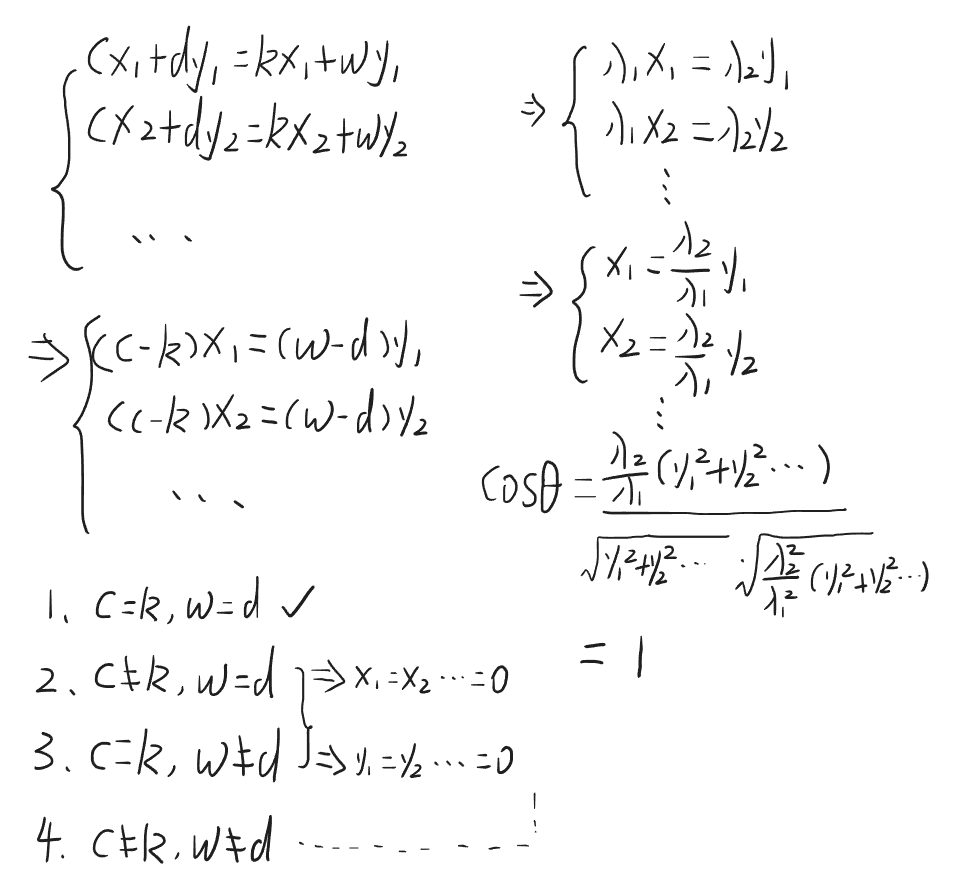
\includegraphics[width=\linewidth ,totalheight=0.95\textheight , keepaspectratio]{线性组合下向量相等的判定.png}
\caption{线性组合下向量相等的判定}
\end{figure}

上面1234四种情况,第一种情况正是我们要证明的,而第二种和第三种情况可以推出某个向量为零向量,这和条件该线性组合可以形成平面冲突。第四种情况可以证明这两个向量的夹角是零,也就是这两个向量是平行的,这也和条件冲突,于是得证。


\subsection{问题集1.1第6题}
\cite{线性代数引论}问题集1.1第6题,作者内心一个潜藏的推理思路是:如果向量的线性组合,可以从中发现某些普遍规律,也就是找到某种关系,使得这个关系不依赖参数c、d...等,那么这个普遍规律对于该线性组合下的所有点都是成立了。【我们太习惯某个事物的局部或者某些特殊情况会更简单一些,常常会忘了在某些时候(这种情况确实很罕见,但也是存在的),该事物从全局从一般情况思考会更简单一些,发现一些普适性的规律,然后自然那些局部的点特殊的情况也一应得到证明了。】

\subsection{问题集1.1第15题}
\cite{线性代数引论}问题集1.1第15题的 $\frac{3}{4}\boldsymbol{v} + \frac{1}{4}\boldsymbol{w}$ 为什么一定在对角线上,证明如下:

\begin{figure}[H]
\centering
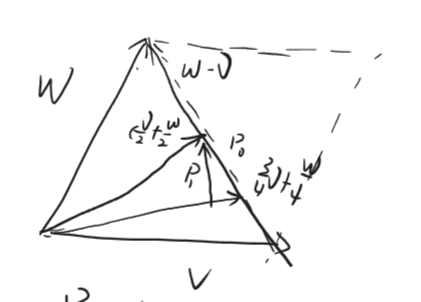
\includegraphics[width=\linewidth ,totalheight=0.95\textheight , keepaspectratio]{线性代数引论问题集1_1_15.png}
\caption{线性代数引论问题集1.1.15}
\end{figure}

已知该对角线为 $\boldsymbol{w} - \boldsymbol{v}$,标记该向量为 $P_0$,现在假定$\frac{3}{4}\boldsymbol{v} + \frac{1}{4}\boldsymbol{w}$ 射出去之后并没有落在对角线上,从而根据$\frac{1}{2}\boldsymbol{v} + \frac{1}{2}\boldsymbol{w}$ 和$\frac{3}{4}\boldsymbol{v} + \frac{1}{4}\boldsymbol{w}$ 的终点确立向量 $P_1$。【已经证明了$\frac{1}{2}\boldsymbol{v} + \frac{1}{2}\boldsymbol{w}$的终点是落在那条对角线的中点的,这很简单,用简单的三角几何分析即可。】

\begin{align*}
P_1 &= \frac{v}{2} + \frac{w}{2} - (\frac{3v}{4} + \frac{w}{4}) \\
    &= -\frac{1}{4}v + \frac{w}{4} \\
    &= \frac{1}{4}(w-v) \\    
 => P_1 // P_0
\end{align*}

因为 $\frac{1}{2}\boldsymbol{v} + \frac{1}{2}\boldsymbol{w}$ 在那条对角线的上,所以 $\frac{3}{4}\boldsymbol{v} + \frac{1}{4}\boldsymbol{w}$ 一定在这条对角线上。上面的证明过程还证明了 $P_1$ 的长度是1/4对角线长度,其终点位置刚好是对角线下面1/4的位置。

上面的证明还可以继续推广,问向量$\boldsymbol{v}$和向量$\boldsymbol{w}$组成的线性组合$c\boldsymbol{v} + d\boldsymbol{w}$ ,$c$和$d$满足何种约束条件就能让其都落在中间那条对角线也就是 $\boldsymbol{w} - \boldsymbol{v}$ 上。

证明如下,其中用到了上面提及的线性组合下向量相等的判定:

\begin{figure}[H]
\centering
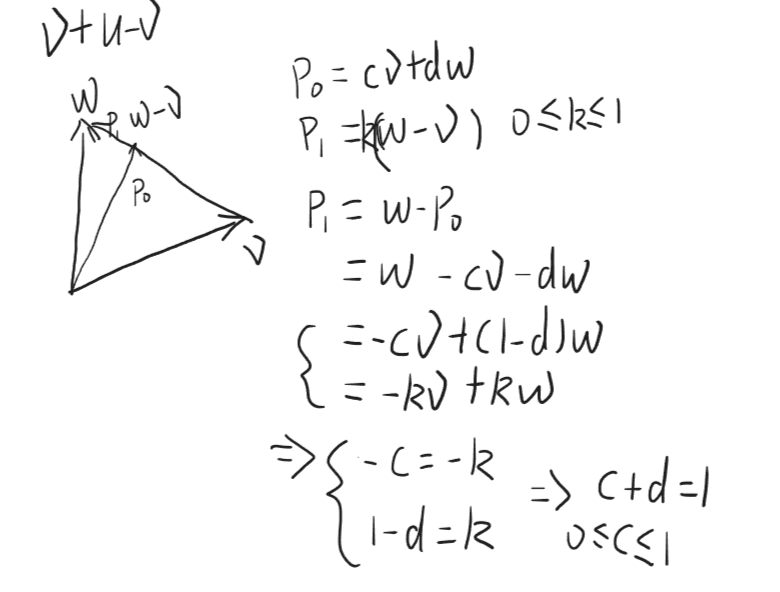
\includegraphics[width=\linewidth ,totalheight=0.95\textheight , keepaspectratio]{线性代数引论问题集1_1_15_2.png}
\end{figure}

最终得证:向量 $P_0 = c\boldsymbol{v}+d\boldsymbol{w}$ ,该向量如果满足 $c+d=1$的条件,则射出去的向量落点会落在中间那条对角线上。


\cite{线性代数引论}问题集1.1第20题将上面讨论的情况扩展到了三个向量的线性组合,问这三个向量的线性组合中,某个向量的系数满足何种条件,该向量的落点在这三个向量终点构成的三角形平面上,有了前面的基础,就很容易得证了。


\begin{figure}[H]
\centering
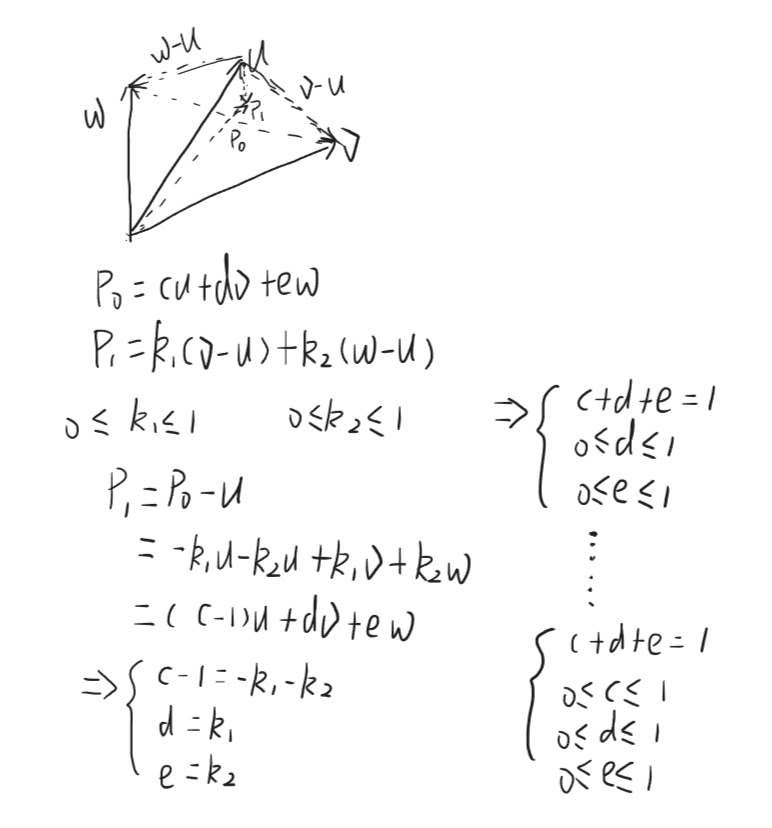
\includegraphics[width=\linewidth ,totalheight=0.95\textheight , keepaspectratio]{线性代数引论问题集1_1_20.png}
\end{figure}


\chapter{术语}
\section{恒等于}
$A \equiv B$ 表示A恒等于B。恒等于仍然是属于 $A=B$的概念范畴,即A和B都是指一个东西。而恒等于是更加精细的等于的说法,A恒等于B的意思是这里仅仅只是用到了一些名称缩写或其他名字上的变化规则,在这里没有任何新的数学知识引入进来。

\section{定义等于}
$A := B$ 表示A定义等于B。定义等于仍然属于 $A=B$的概念范畴,只是更加精细地表明了在这里是先验地定义或者说假定这个语句为真。比如说 $x := x*x$ ,该语句的意思是假定x的值被定义等于其自身的平方。在后续的讨论中$x$当然等于$x*x$,只是更加精细地指出这个等于语句是先被假定为真的。


\section{当且仅当}
当且仅当的英文是if and only if,常缩写为iff。

A当且仅当B:如果A成立则B成立 ,并且如果A不成立则B不成立【等价于如果B成立则A成立】。

如果命题只有真或者假两种可能性,在所有情况下真值都相同,所以A不成立则B不成立等价于如果B成立则A成立。

\begin{table}[H]
\begin{tabular}{@{}llllll@{}}
\toprule
{A} & {B} & {¬A} & {¬B} & {¬A→¬B} & {B→A} \\ \midrule

{T}          & {T} & {F}  & {F}  & {T}     & {T}   \\
\rowcolor[HTML]{FFFFFF} 
{T}          & {F} & {F}  & {T}  & {T}     & {T}   \\
\rowcolor[HTML]{FFFFFF} 
{F}          & {T} & {T}  & {F}  & {F}     & {F}   \\
\rowcolor[HTML]{FFFFFF} 
{F}          & {F} & {T}  & {T}  & {T}     & {T}   \\ \bottomrule
\end{tabular}
\end{table}


\section{自然数集}
本文认为0不属于自然数集,当本文讨论自然数集 $ \mathbb{N} $的时候,等于正整数集 $\mathbb{N}^{*}$,即本文认为:

\[
\mathbb{N} \equiv \mathbb{N}^{*}
\]


\chapter{约定}
向量一般默认为列向量。可以写为 $(x_1, x_2...)$ 或者 :

\[
\begin{bmatrix}x_{1}  \\ x_2 \\ \vdots \end{bmatrix}
\]

行向量则写为 $[x_1, x_2...]$


\part{附录:编程知识}
编程知识介绍以markdown或者ipynb notebook的形式散落各处,而且只关注介绍28法则中那些最常用最核心的知识点,集中学习一段时间即可,后续应用中若用疑问可搜索可问AI或者查看官方文档等。


\chapter{python语言核心教程}
\href{https://a358003542.github.io/articles/python-core-tutorial.html}{python语言核心教程}



\chapter{numpy基础}
\href{https://github.com/a358003542/ipynb_notebook/blob/master/linear_algebra/numpy_basic.ipynb}{numpy basic}


\chapter{pandas基础}
\href{https://github.com/a358003542/ipynb_notebook/blob/master/linear_algebra/pandas_basic.ipynb}{pandas basic}

\chapter{matplotlib基础}
\href{https://github.com/a358003542/ipynb_notebook/blob/master/matplotlib_basic.ipynb}{matplotlib basic}

\chapter{pytorch基础}
\href{https://github.com/a358003542/ipynb_notebook/blob/master/neural_network/pytorch_basic.ipynb}{pytorch basic}

\backmatter
\part*{附录:参考资料}
\begin{thebibliography}{99}
\bibitem[线性代数引论]{线性代数引论} 《Introduction to Linear Algebra 5e》 by Gilbert Strang at 2016 .
\bibitem[Dive into Deep Learning]{Dive into Deep Learning} 《Dive into Deep Learning》 by Aston Zhang \& Zachary C. Lipton \& Mu Li \& Alexander J. Smola at 2023.
\bibitem[什么是数学]{什么是数学} 《什么是数学:对思想和方法的基本研究(第三版)》 by [美] R·柯朗 \& H·罗宾 \&  左平  at 2012.
\bibitem[Elements of Set Theory]{Elements of Set Theory} 《Elements of Set Theory》by Herbert B. Enderton at 1977.
\bibitem[人工智能:现代方法]{人工智能:现代方法} 《人工智能:现代方法(第4版)》by [美]斯图尔特·罗素 \& [美]彼得·诺维格 at 2023.
\bibitem[烧掉数学书]{烧掉数学书} 《烧掉数学书:重新发明数学》by [美]杰森·威尔克斯 \& 唐璐 at 2020.
\end{thebibliography}
\end{document}


